\section{Introduction}

We've already seen some of the properties of DC~circuits; as you'll recall, in 
a DC~circuit, the current and voltage values are steady.  A much more general 
situation is where the voltage and current values change over time, as is the 
case with the power supplied by the wall outlets in our homes and in our 
laboratory.  The voltage and current supplied by a wall outlet does not change
arbitrarily, however. They are examples of {\it periodic} signals, they repeat 
themselves over time; for outlets in the US, the frequency of oscillation is 
60~Hz.  

Since these periodic signals are so important to us (our appliances, computers,
TV's, etc.\ use them), we will spend a few weeks studying examples of 
AC~circuits with varying types of periodic signals. We'll learn some crucial
fundamental principles along the way. It is important that we learn how to 
make measurements with such circuits; this will be our goal for this week's 
lab.  The device we'll use, an oscilloscope, will display on its screen a 
visual representation of the signal produced by the changing voltage across a 
part of our circuit. We can measure the period of a signal, read off voltage 
values at specific times along the signal, and display two signals so that we 
can compare them.  Viewing two signals will be important when we want to 
learn how the output from a specific device, such as an inductor or capacitor, 
depends on the characteristics of the input signal. 
\vfill
\pagebreak

\section{Theory}

\subsection{References}

The properties of waves are discussed in Serway, Chapter~16 (Wave Motion). 
 

\subsection{The Properties of Waves}
\label{sec:SCOPE:waveprop}
As we mentioned in the introduction, a signal which repeats itself after a 
certain amount of time is called {\it periodic}; such a signal is shown in 
Figure~\ref{fig:scope:periodic}.
\begin{figure}[htb]
\centering \epsfxsize=12cm 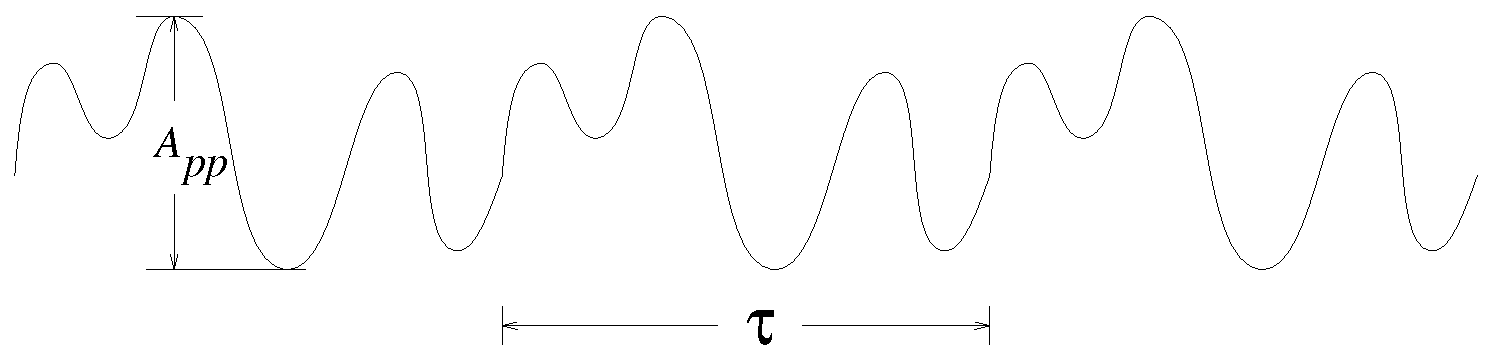
\includegraphics[scale=0.5]{4_oscilloscope/periodic.eps}
\caption{A periodic, albeit weird, signal.}
\label{fig:scope:periodic}
\end{figure}
The amount of time it takes for the signal to repeat is called the {\it period}
of the signal and is denoted $T$.  The {\it rate} at which 
the signal repeats itself is called the {\it frequency} and is denoted by $f$. 
It is easy to see that $f=1/T$.  The maximum ``height'' between the peaks of
the signal is called the {\it peak-to-peak amplitude} and denoted $A_{pp}$.
What we more commonly refer to as the {\it amplitude} is half of $A_{pp}$.  

The periodic signals we will study are often referred to as {\it waves}, due to
their relationship to the physically important solutions to the {\it wave
equation}.  The first type of wave we'll discuss is the sinusoid in 
Figure~\ref{fig:scope:sinusoid}.
\begin{figure}[!htb]
\centering \epsfxsize=8cm \includegraphics[scale=0.5]{4_oscilloscope/sinusoid.eps}
\caption{A sinusoidal wave.}
\label{fig:scope:sinusoid}
\end{figure}
The mathematical functions that describe sinusoidal waves are sine and cosine.
They can be expressed in the form
\begin{eqnarray*}
& F(t) = A \sin(\omega t+\phi) & \\ 
& \mbox{or} & \\
& F(t) = A \cos(\omega t+\theta), &  
\end{eqnarray*}
where $\omega$ is the {\it angular frequency}, defined by $\omega=2\pi f$, and
$\phi$ and $\theta$ are constants called {\it phase angles}.  The phase angle
is an artifact of the time-coordinate we choose to define the sinusoid; it
tells us where the zeros of the wave are located.  Since the sine and cosine
functions take a maximum value of 1, we see that $A$ is the {\it amplitude} of 

the wave.

The concept of phase is an important one; we'll learn how to measure the 
{\it difference} in phase between two waves in the lab. Let's examine an 
example: the phase difference between sine and cosine waves of the same 
frequency, 
illustrated in Figure~\ref{fig:scope:phasediffer}, where
\begin{eqnarray*}
& F_1 & =A_1\sin\omega t,  \nonumber \\
& F_2 & = A_2 \cos\omega t.
\end{eqnarray*}
\begin{figure}[htb]
\centering \epsfxsize=8cm \includegraphics[scale=0.5]{4_oscilloscope/phasediffer.eps}
\caption{Sine and cosine waves differ in phase.}
\label{fig:scope:phasediffer}
\end{figure}
We see that these two waves differ along the time axis; that the amplitudes
are different does not matter; the maxima, minima, and zeros of the two waves
will always differ by a distance in {\it time}, $\Delta t$, called the 
{\it phase difference} between 1 and 2.  We note that it is important that the 
two waves are of the {\it same} frequency. If we were dealing with waves of 
different frequencies, as in Figure~\ref{fig:scope:differfreq},
\begin{figure}[htb]
\centering \epsfxsize=8cm \includegraphics[scale=0.5]{4_oscilloscope/differfreq.eps}
\caption{The concept of phase difference does not apply to waves of different
frequencies.}
\label{fig:scope:differfreq}
\end{figure}
there's no reason for the maxima (or minima, or zeros) to be separated by a 
{\it uniform} amount.  The concept of phase difference is, therefore, 
meaningless unless we are discussing waves of the same frequency.

Let's see how phase difference relates to the concept of phase angle. Again 
we'll study the sine and cosine example. Note that, from the trigonometric
identity
$$ \sin(A+B) = \sin A \cos B + \cos A \sin B, $$
we can write
$$ \cos\omega t = \sin (\omega t +90^\circ), $$
where $90^\circ$ is a phase angle.  We can therefore write
\begin{eqnarray*}
& F_1 & = A_1 \sin \omega t \nonumber \\
& F_2 & = A_2 \sin(\omega t+90^\circ).
\end{eqnarray*}
These are of the same functional form (though of differing amplitudes), but 
differ in that the phase angle of $F_2$ is $\phi_2=90^\circ$, while that of 
$F_1$ is $\phi_1=0$.  In a more general case, we might have
\begin{eqnarray*}
& F_1 & = A_1 \sin (\omega t+\phi_1) \nonumber \\
& F_2 & = A_2 \sin (\omega t + \phi_2);
\end{eqnarray*}
the {\it angular phase difference} between 1 and 2 is defined to be
$$ \phi=\phi_2-\phi_1.$$  
We note that a similar definition exists if we have cosine, rather than sine, 
waves. As an exercise, the student should verify that the time shift, 
$\Delta t$, is related to the angular phase difference, $\phi$, by
\begin{equation}
\fbox{$ \displaystyle \frac{\phi}{2\pi} = \frac{\Delta t}{T}.$} \label{eq:scope:angphase}
\end{equation}

Another type of wave that we'll find important is the {\it square wave}, 
illustrated in Figure~\ref{fig:scope:squarewave}.
\begin{figure}[htb]
\centering \epsfxsize=8cm 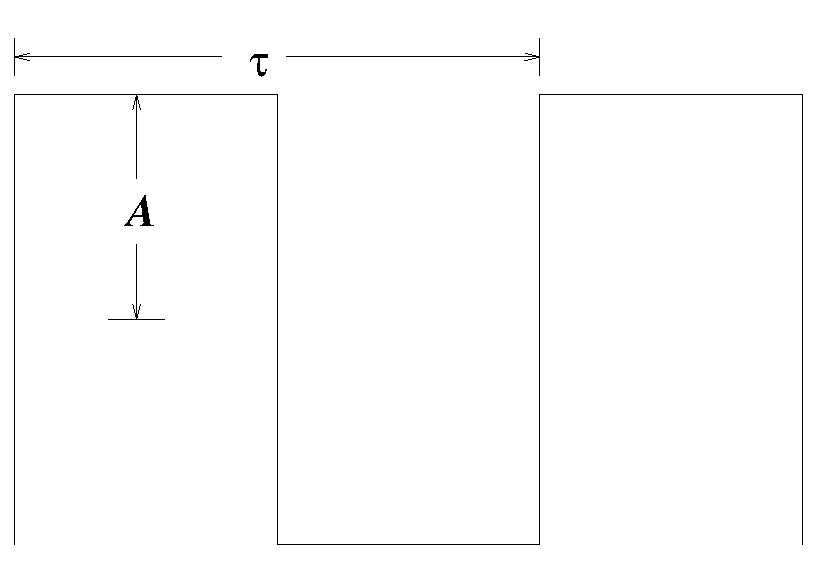
\includegraphics[scale=0.6]{4_oscilloscope/squarewave.eps}
\caption{A square wave.}
\label{fig:scope:squarewave}
\end{figure}
Functionally, we can write
$$ F(t) = \left\{ 
\begin{array}{cc} A & 0<t<T/2 \\ -A & T/2<t<T. \end{array} \right. $$
The concept of phase difference (but not phase angle, this isn't a 
trigonometric function!) can clearly be applied to two square waves of the same
frequency, see Figure~\ref{fig:scope:squarephase}.
\begin{figure}[htb]
\centering \epsfxsize=8cm 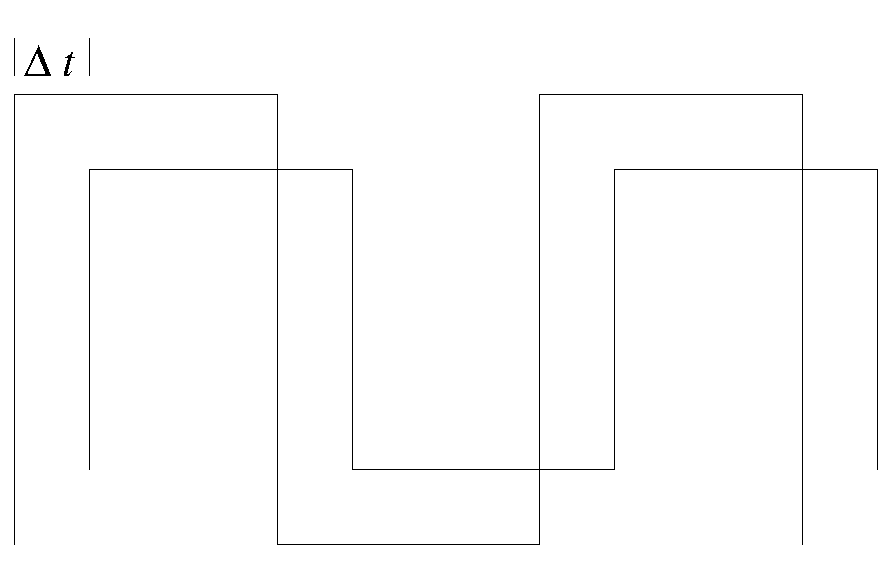
\includegraphics[scale=0.6]{4_oscilloscope/squarephase.eps}
\caption{A phase difference between two square waves.}
\label{fig:scope:squarephase}
\end{figure}
Finally, we also have the {\it triangle wave} in 
Figure~\ref{fig:scope:triwave}.
\begin{figure}[htb]
\centering \epsfxsize=8cm 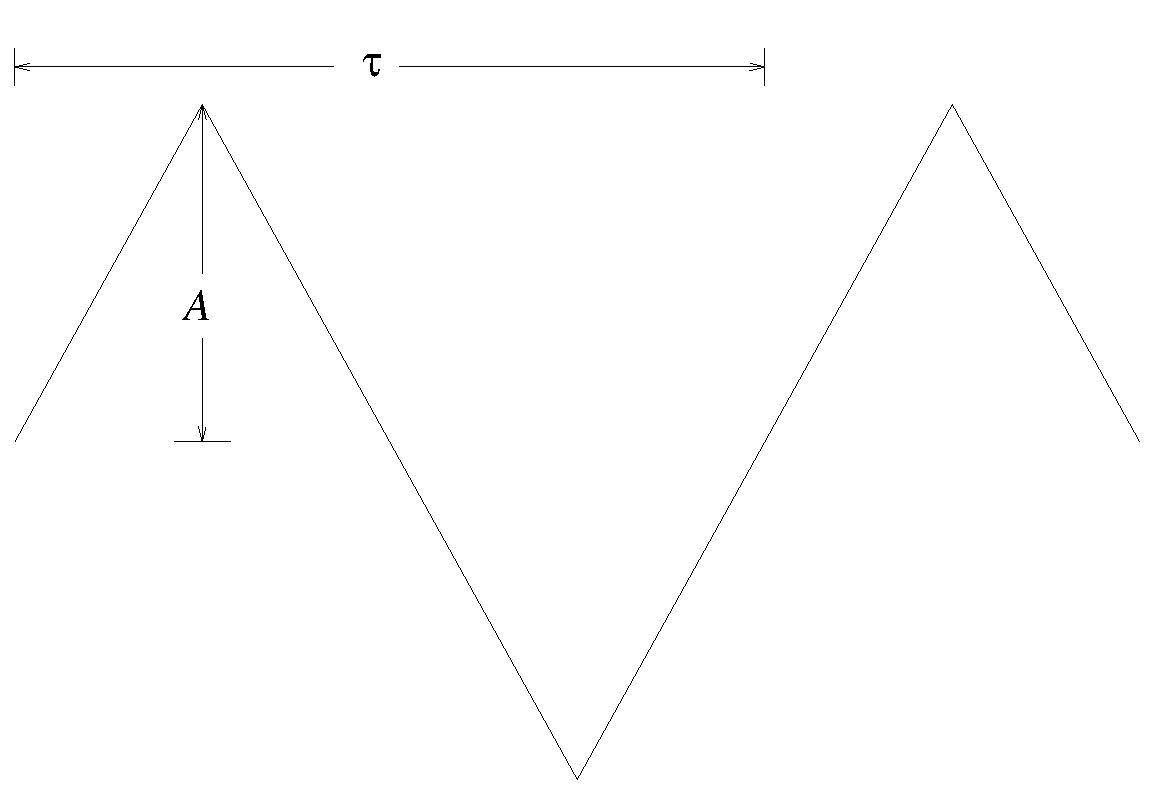
\includegraphics[scale=0.4]{4_oscilloscope/triwave.eps}
\caption{A triangle wave.}
\label{fig:scope:triwave}
\end{figure}
We leave it to the interested student to write the triangle wave down in 
mathematical form. Note that, once again, phase difference is meaningful for
triangle waves of equal frequency.

\section{Apparatus}

\subsection{The Oscilloscope}

The oscilloscope is a device which displays a voltage signal, constant or 
time-varying, periodic or otherwise, as a function of time.  What this amounts
to is an extremely enlightening picture of what is happening in our circuit.
The ability to adjust the characteristics of how the oscilloscope displays our
signal makes it an extremely versatile tool.  An illustration of the 
oscilloscope we'll be using appears in Figure~\ref{fig:scope:oscope}.
\begin{figure}[htb]
\centering \epsfxsize=16cm \includegraphics[scale=0.05]{4_oscilloscope/TDS1002FP.eps}
\caption{The Tektronix model TDS1002 oscilloscope.}
\label{fig:scope:oscope}
\end{figure}

How does the oscilloscope work? Everything starts with a signal fed
into one of the channels of the oscilloscope. The idea is to get a voltage
versus time representation of that signal on the screen of the instrument. The
screen of the scope is therefore scanned from left to right at a constant
speed and the voltage at each instant is displayed as a vertical deviation from
the horizontal axis. Since the screen has a limited width, this scan will end
in a finite amount of time. Then, to keep giving current information on our
signal, the instrument has to erase the screen and start scanning again. Now
imagine that happening many times in a second. In general, every scan would
create a different $V$ vs. $t$ graph and we would just see a blur of many
different waveforms displayed rapidly one after another. For periodic signals,
this situation can be amended if the scanning always starts from the same
position on a cycle of the wave. Imagine for instance a sinusoidal waveform.
If the oscilloscope could somehow ``understand'' that it should always start
scanning when the voltage crosses zero, going from negative to positive
values, then the same waveform would be presented over and over again on the
screen. We would be looking then at a stable picture, like the one in
Figure~\ref{fig:scope:sinusoid}. This is a picture we can study.

To make the oscilloscope ``understand'' where on a signal it should start
scanning, we use a logic circuit, called the {\it trigger}. More formally, a
trigger is configured to set a time origin, for each scan of the acquired
signal. The signal displayed on the screen starts a set amount of time before
this time origin. There are many ways to implement triggering. In this lab, we
are going to be using {\it edge triggering}. In this method, the trigger is
waiting for the signal to raise or drop to a set value, called the {\it trigger
level}. The acquired signal is displayed on the screen, so that this event always
determines the horizontal axis origin (the time $t=0$, which doesn't necessarily
coincide with the horizontal axis midpoint). The example with the sinusoidal wave
(see previous paragraph) illustrates edge triggering.

How do we make measurements with the oscilloscope? The oscilloscope display,
as can be seen in Figure ~\ref{fig:scope:dscope}, provides a system of axes,
each one of which has large and small divisions on it.
The vertical direction indicates the voltage value of the input at a given 
time; each of the eight large divisions indicates a number of volts given by the
V/div scale factor on screen.  For example, if we measure the amplitude of 
the signal displayed to be 3.6~div (ignoring uncertainty for the moment)
and if the V/div scale factor is set at 0.5~V/div, then the amplitude,
in volts, is 
$$ (3.6~\mbox{div}) (0.5~\mbox{V/div}) = 1.8~\mbox{V}. $$
We should always use the V/div scale factor so that we report the amplitude, and
any other voltage values we measure, in units of voltage. The horizontal direction
indicates time; there are ten large divisions. If we measure the distance between 
the maxima of a sinusoidal wave to be $5$~div and the sec/div scale factor
reads 5~ms/div, then the period is 
$$(5~\mbox{div}) (5~\mbox{ms/div}) = 25~\mbox{ms}.$$

What about the uncertainty in our measurements made with the oscilloscope? 
Note that, since the oscilloscope screen is ruled, the finest scale marking 
may be used to estimate the uncertainty in all of the measurements we make.  
Estimating the uncertainty in this manner is precisely the same thing we do
when we're measuring length with a ruler. Remember that the uncertainty 
expressed in divisions, like the quantity itself, must be multiplied by the 
proper scale factor to obtain an uncertainty expressed in the appropriate 
units.

With a digital oscilloscope, like the one we will be using, measurements can
be facilitated by screen aids. In this lab, these aids take the form of pairs
of horizontal and vertical lines, called {\it cursors}. The position of each
line can be adjusted by the user, and is displayed, along with their separation,
on the oscilloscope screen. By using one line as a voltage or time reference,
we can use the other, to find the voltage or time at any point on the
displayed signal. Since all cursor positions and distances from each other are
given on the screen as digital readings, the uncertainty for each number will
be its increment of change.

In this lab we will be using the Tektronix TDS1002 digital oscilloscope.
The interface of this instrument with its operator comprise: a set of
single function knobs (the large VOLTS/DIV and SEC/DIV knobs) and buttons
(all the labeled buttons), a set of multi-function knobs (the smaller
POSITION and LEVEL knobs) and buttons (the unlabeled, option buttons on the
side of the screen), as well as the screen-displayed information and menus.
The following description focuses on controls and display items that are going
to be needed for our experiments. 

\begin{enumerate}

\begin{figure}[htb]
\centering \epsfxsize=16cm 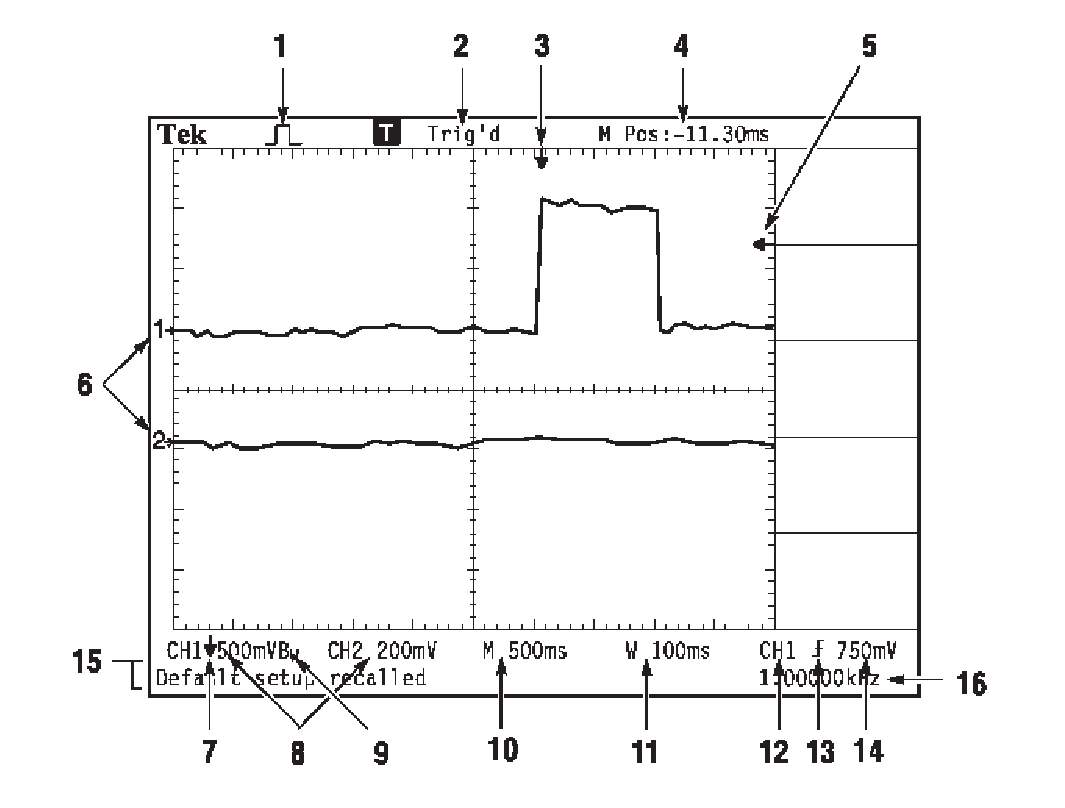
\includegraphics[scale=0.7]{4_oscilloscope/tds1002d.eps}
\caption{The Tektronix model TDS1002 oscilloscope display.}
\label{fig:scope:dscope}
\end{figure}

\item {\bf The Display}

A typical oscilloscope display is shown in
Figure ~\ref{fig:scope:dscope}. The indicators of interest to us are:

\begin{itemize}

\item[3.] Trigger position (time origin).

\item[4.] Center of horizontal axis position. Observe that the time origin
does not coincide with the center of the time axis. The HORIZONTAL POSITION
knob can move the origin, and therefore the waveform, on this axis.

\item[5.] Edge trigger level.

\item[6.] Ground reference levels for each channel. If one of these indicators
is missing, the corresponding channel is not displayed.

\item[8.] Vertical scale factors for each channel. The values correspond to
the large divisions of the vertical axis

\item[10.] Horizontal scale factor. The value corresponds to the large
divisions of the horizontal axis. Observe that the time scale is the same for
both channels.

\item[16.] Trigger frequency. This should in general agree with the frequency
of our signals. It may be used as a verification of our calculations, but not
as a direct measurement.

\end{itemize}

On the right side of the screen, there is a dynamic menu, indicating the
function of the adjacent, unlabeled, option buttons. These functions change,
every time a different menu button is pressed on the control panel.

\item {\bf Vertical Controls}

{\bf VOLTS/DIV knobs:} They adjust the vertical axis scale factor for each
channel.

{\bf POSITION - CURSOR knobs:} They adjust the ground reference level, in
effect moving the corresponding waveform vertically on the screen. When the
cursor menu is active, the LEDs below them are illuminated, indicating that
the knobs now set the cursor line positions.

{\bf CH MENU:} Display the vertical menu and toggle the corresponding
channel on and off. The vertical menu for each channel contains two functions
that we will find useful.

\begin{enumerate}

\item {\bf Coupling:} Determines what part of a signal is shown on the screen
The possible choices here are:

{\bf AC:} Only the alternating part of the signal is displayed. Any constant (DC)
offset is filtered out.

{\bf DC:} The signal is displayed unfiltered.

{\bf GND:} The input is connected to a zero voltage reference. The oscilloscope
output is a horizontal line at the ground reference level.

\item {\bf Probe:} Sets multiplicative factors for the acquired voltages. This is
done to accommodate the use of special probes. {\bf The default setting is
10X. You must switch to a 1X setting, since we are not using a special probe for
our measurements.}

\end{enumerate}

\item {\bf Horizontal Controls}

It should be noted that these controls affect settings which are common to both
channels.

{\bf SEC/DIV knob:} It adjusts the horizontal axis scale factor for both
channels.

{\bf POSITION - HELP SCROLL:} In all but the help mode, this knob adjusts the
horizontal position of the displayed signals on the screen. It does that by
varying the position of the center of the horizontal axis with respect to the
time origin.

{\bf SET TO ZERO:} Makes the time origin coincide with the center of the
horizontal axis.

{\bf HORIZ MENU:} Displays the horizontal menu. The only function of potential
use to us here is the {\bf Trig Knob} option. This allows us to toggle the
TRIGGER LEVEL knob between its default function of setting the trigger level and
a secondary function of adjusting the trigger holdoff. The trigger holdoff is the
smallest possible interval between two successive triggerings of the oscilloscope.
It may be used to stabilize a waveform on the screen.

\item {\bf Trigger Controls}

The controls we are most commonly going to use are:

{\bf TRIGGER LEVEL:} Sets the voltage that the trigger signal has to cross, for
triggering to occur.

{\bf TRIG MENU:} Displays the trigger menu. There are three options that we may
find useful.

\begin{enumerate}

\item {\bf Edge/Video/Pulse:} Defines triggering type. By default, edge triggering
is, and should remain, selected.

\item {\bf Source:} Allows us to select the source of the triggering signal. You
may have to adjust it, to make sure it corresponds to your reference channel
(CH1 or CH2).

\item {\bf Slope:} Determines whether the trigger level has to be crossed while
the signal rises or falls. This control allows us to get the desired portion of
the signal displayed.

\end{enumerate}

\item {\bf Menus}

{\bf CURSOR:} This is the only menu we are going to use from this group. The
cursors are pairs of vertical or horizontal lines that allow us to perform
time or voltage measurements respectively. The items on the on-screen menu
are described below.

\begin{enumerate}

\item {\bf Type:} Toggles between voltage, time, or no cursors.

\item {\bf Source:} Selects the channel for which measurements are to be
performed.

\item {\bf Delta:} The difference in the position of the two cursors.

\item {\bf Cursor 1:} Cursor 1 position. The time origin is set by the
trigger, while the voltage origin is the ground reference level.

\item {\bf Cursor 2:} Cursor 2 position. Time and voltage origins are the same as
for Cursor 1.

\end{enumerate}

\item {\bf DEFAULT SETUP}

The DEFAULT SETUP button should be used at the beginning of each lab as well as
whenever you feel uncomfortable or unsure about the oscilloscope settings. The
factory defaults provide a good start and protect you from time-consuming
guesswork. You should note that, by default, the oscilloscope uses a 10X
multiplier for its inputs. {\bf YOU HAVE TO MANUALLY SELECT THE 1X SETTING FROM
THE CH1 AND CH2 MENUS EACH TIME YOU RECALL THE DEFAULT SETUP.} Failure to do so
will lead to erroneous measurements.

\end{enumerate}

\subsection{The Function Generator}

The function generator is designed to produce waveforms of variable shape,
frequency, and amplitude; an illustration of a typical one appears in
Figure~\ref{fig:scope:functiongen}.
\begin{figure}[htb]
\centering \epsfxsize=14cm 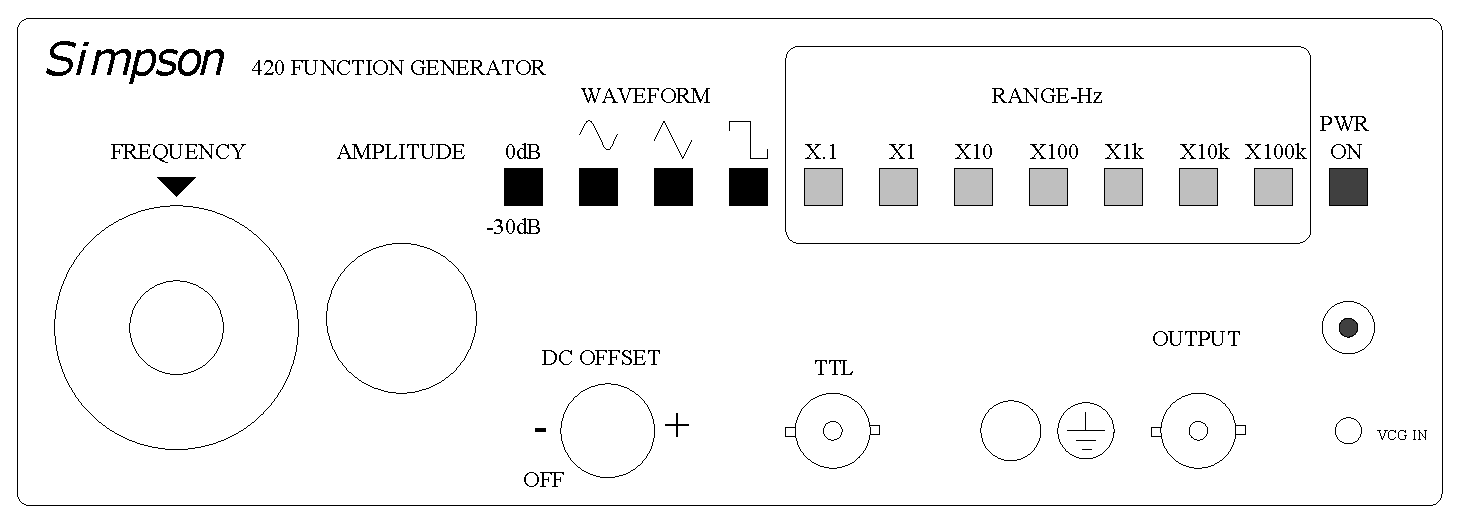
\includegraphics[scale=0.5]{4_oscilloscope/functiongen.eps}
\caption{The function generator.}
\label{fig:scope:functiongen}
\end{figure}
The function generator controls are as follows:

\begin{enumerate}

\item {\bf power}: This button just turns the function generator on and off.

\item {\bf output}: This BNC connection is the signal output.

\item {\bf waveform}: These buttons select between sinusoidal, triangle, or 
square wave output.

\item {\bf amplitude}: This adjusts the amplitude (voltage value) of the output
signal.

\item {\bf 0~dB/-30~dB}: This button selects between two output voltage ranges.
We'll want to keep this on the 0~dB setting, for a strong output signal.  

\item {\bf frequency}: This allows for fine tuning of the frequency output.
The maximum on the dial corresponds to the value indicated by the range
setting switches (see below.) The frequency read from the function 
generator should be regarded as a strictly nominal value. Since we generally 
want a frequency value that we can trust, we will {\it always} be sure to 
measure the frequency with the oscilloscope; we don't want to place very much 
trust in the nominal value.

\item {\bf range}: These buttons select between available frequency ranges. In
our case, from 0.2~Hz to 2~MHz.

\item {\bf DC offset}: This provides a DC component to the output signal. Since
we'll only be interested in AC signals, we'll leave this set to {\it off}.

\end{enumerate}

\subsection{The Phase Shifter}

The phase shifter consists of a variable resistor and two capacitors, 
illustrated in Figure~\ref{fig:scope:phaseshifter}.
\begin{figure}[htb]
\centering \epsfxsize=8cm 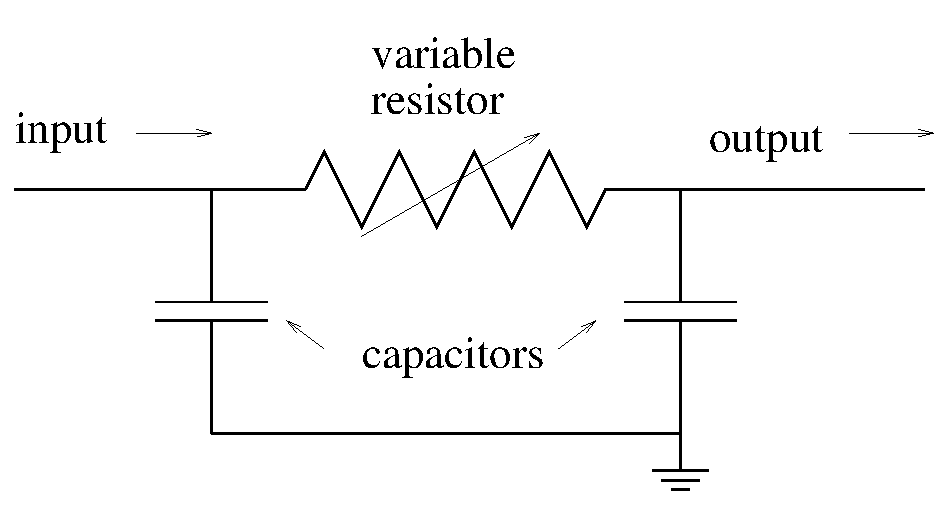
\includegraphics[scale=0.5]{4_oscilloscope/phaseshifter.eps}
\caption{The phase shifter circuit.}
\label{fig:scope:phaseshifter}
\end{figure}
The knob on the phase shifter box controls the amount of resistance provided
by the variable resistor.  When we study RC circuits in the next lab, we'll
learn that these circuits change both the {\it amplitude} and {\it phase} of
an AC input, but not its frequency.  For now, we can ignore the details of
why this happens; we'll simply use the phase shifter to change the phase of the
output signal.  By examining the input and output signals together on the 
oscilloscope, we'll learn how to measure phase differences between signals.

\vfill
\pagebreak
$$
$$
\vfill
\clearpage
\newpage


%  Label worksheets by \thechapter.W
\renewcommand{\thesection}{\thechapter.W}

\section{Oscilloscope Worksheet}

{\bf \Large Name:}~ \rule{5cm}{.1mm}~~~~~~~
{\bf \Large Day/Time:}~\rule{3cm}{.1mm}\\
{\bf \Large Partner's Name:}~\rule{6cm}{.1mm}\\
   \subsection{In-Lab Procedure}

\subsubsection{Turning on the Oscilloscope}
\label{sec:scope:ground}
Turn on the oscilloscope and wait until the trace appears. Reset the settings
of the instrument by pressing the DEFAULT SETUP button. Don't forget that,
every time you do that, you have to switch the Probe setting in {\it each}
channel's menu to 1X. The procedure may sound tedious, but it will save you
time and elliminate the frustration of guessing what's wrong with the settings
of your instrument. Feel free to repeat it any time the readings of the
oscilloscope don't make sense.

\subsubsection{Operating the Equipment}
\label{sec:scope:oper}
Now that the oscilloscope has been reset, turn the function generator on and 
connect it to one of the channels.  Set it to produce a sinusoidal wave of 
approximately~1~kHz; the amplitude should be set to an arbitrary non-zero 
value. Make sure that the channel's Coupling option is set to DC and that 
you are triggering on the channel that you've connected the input to. Adjust 
the V/div and sec/div knobs so that a single wave fills the screen,
%as illustrated in Figure~\ref{fig:scope:oscope}.
This means that no more than two cycles (and no less than one cycle) of the
signal should appear and that the vertical size of the waveform should be as
large as possible on the oscilloscope screen.  The controls of the instrument
are versatile enough to allow you to adjust the display so that you can
comfortably make measurements of the amplitude and period of the signal.

\noindent Check that the sine wave appears to be symmetric about the
horizontal axis; if not, you need to adjust the vertical position. To do this,
you do not need to disconnect the input. Simply set the channel's Coupling
option to GND and use the vertical position knobs to realign the trace with the
axis. You might need to repeat this procedure again later, since changing the
V/div and sec/div scales can upset the ground. When you're done, be sure to
return the Coupling option to DC.

\noindent Before making any measurements, let's experiment with the equipment a
bit. Change the amplitude and frequency on the function generator and watch how
the signal changes on the screen. Practice readjusting the oscilloscope scales
so that you get only one or two cycles on the screen; readjust the ground when 
necessary.  Now set the function generator to display a square wave.  Again,
experiment with different frequencies and amplitudes. Examine the {\it shape}
of the signal carefully.  You should have a single period filling the screen
before examining the shape, i.e. a change in frequency does not constitute a 
change in shape. \\

\noindent {\bf {\large Answer the following questions completely (not yes or
no) stating your reasoning behind each answer.}}  \\
\\
\noindent {\bf Question 1:} \hspace*{0.5cm} Comparing with 
Figure~\ref{fig:scope:squarewave}, does the shape vary with the frequency?
Illustrate as necessary. \\
\vspace*{2cm} \\  
\noindent {\bf Question 2:} \hspace*{0.5cm}Also examine the triangle waves
produced by the function generator; compare the triangle waves to those
illustrated in Figure~\ref{fig:scope:triwave}.  Does the shape vary with the
frequency? Illustrate as necessary. \\
\vspace*{2cm} \\   
\noindent {\bf Question 3:} \hspace*{0.5cm}  Now make a definitive statement
about the quality of the signals generated by your function generator.  You
will need to use this information as we continue with the labs. \\  

\subsubsection{Measuring Amplitude and Frequency}
\label{sec:scope:measampfreq}

Reset the function generator to produce a sinusoidal wave and adjust the scope
so that the signal fills the screen. You may find it easier to switch the
coupling to AC for the remainder of this lab.  Sketch the wave displayed onto
the grid below.  Use the second grid in case you make a mistake on the first
one.

\begin{center}
\begin{tabular}{ccc}
\epsfxsize=7cm 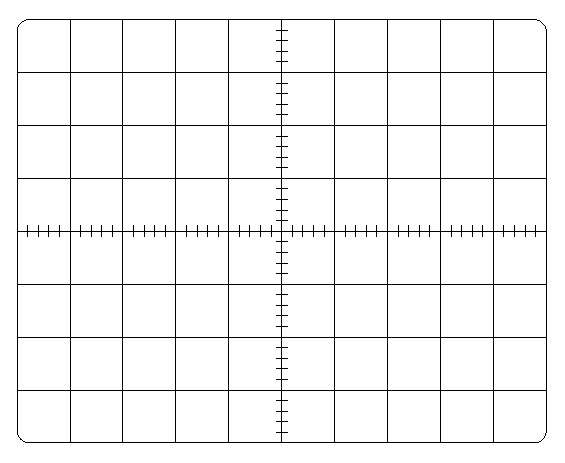
\includegraphics[scale=0.7]{4_oscilloscope/scope.eps} & \hspace{0.5cm} &

\epsfxsize=7cm 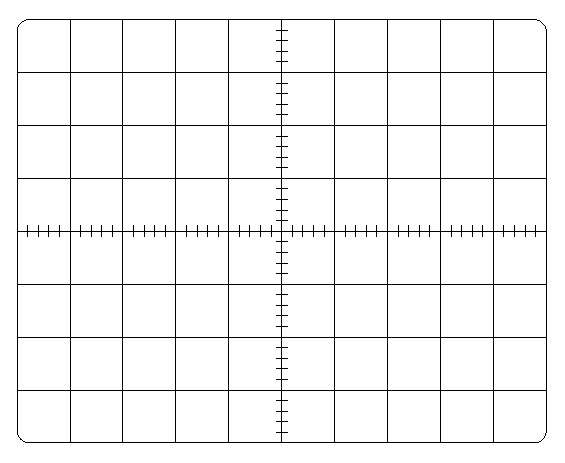
\includegraphics[scale=0.7]{4_oscilloscope/scope.eps}
\end{tabular}
\end{center}
\noindent Record the frequency setting on the function generator in the {\bf
correct units} (Note that this is a nominal value and may be far from the
accurate one): \\
\\
Frequency setting: \rule{3cm}{.1mm}\\
\\
Also recored the V/div and sec/div scales.\\
\\
V/div:  \rule{3cm}{.1mm} \hspace*{1cm} sec/div: \rule{3cm}{.1mm}\\
\\
Using the voltage and time cursors, measure the amplitude and period of the
signal. The easiest and most accurate way to facilitate the cursors for your
measurements is to record their distance (Delta) rather than their absolute
positions. Therefore, if you are measuring period, switch the cursor Type
option to time, place one cursor at the beginning of a cycle and the other at
its end. Delta is then the period of the wave. The uncertainty for all cursor
measurements will be the smallest increment of change in Delta. For the
amplitude you should measure the {\it peak-to-peak amplitude} and divide by
two; this eliminates any error that might creep in if the wave is not symmetric
about the horizontal axis.
% Show all of your work in the space above the answer.
\\
\vfill
Amplitude:  \rule{3cm}{.1mm} \hspace*{1cm} Period: \rule{3cm}{.1mm}\\
\pagebreak

Readjust both the voltage and time scales of the oscilloscope ({\it not} the
function generator settings) so that the signal no longer fills the screen. Be
sure that several cycles can be seen.  Sketch the signal on the grid below.
\begin{center}
\begin{tabular}{ccc}
\epsfxsize=7cm 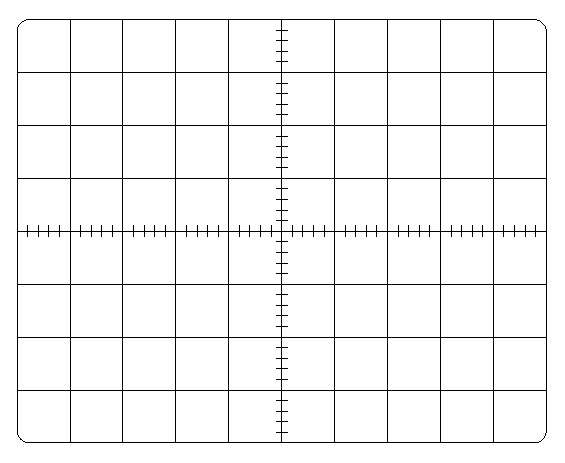
\includegraphics[scale=0.7]{4_oscilloscope/scope.eps} & \hspace{0.5cm} &
\epsfxsize=7cm 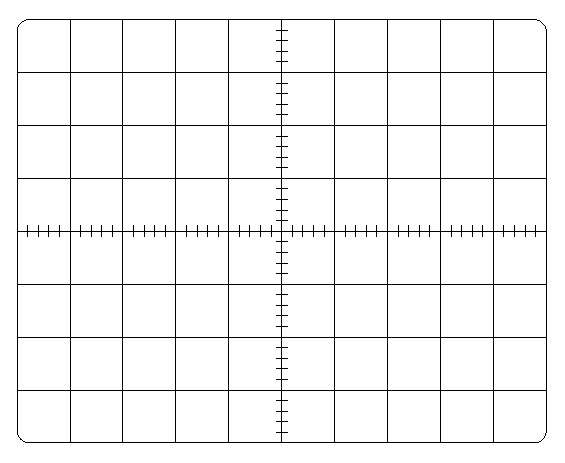
\includegraphics[scale=0.7]{4_oscilloscope/scope.eps}
\end{tabular}
\end{center}
\noindent Recored the V/div and sec/div scales.\\
\\
V/div:  \rule{3cm}{.1mm} \hspace*{1cm} sec/div: \rule{3cm}{.1mm}\\
\\
%\noindent Record the frequency setting on the function generator in the 
%{\bf correct units}: \\
%\\
%Frequency setting: \rule{3cm}{.1mm}\\
%\\
Measure the amplitude and period with units and uncertainties.
% showing your work in the space above your answer.  
\vfill
Amplitude:  \rule{3cm}{.1mm} \hspace*{1cm} Period: \rule{3cm}{.1mm}\\
\pagebreak
\subsubsection{Measuring Phase Difference}
\label{sec:scope:measphdiff}

Let's examine the effect of the phase shifter. Use the BNC T-connector to 
split the output of the function generator. Connect one wire to channel~1 and
the other to the input of the phase shifter.  Connect the output of the phase
shifter to channel~2; the circuit is illustrated in 
Figure~\ref{fig:scope:phasemeas}.
\begin{figure}[htb]
\centering \epsfxsize=8cm 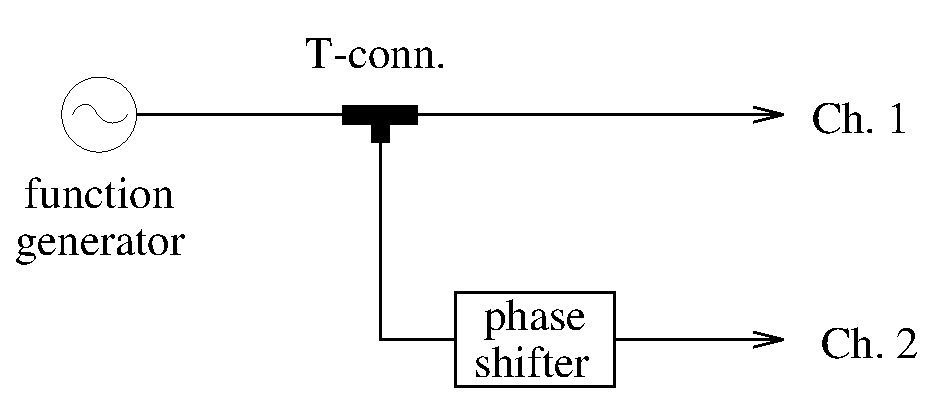
\includegraphics[scale=0.5]{4_oscilloscope/phasemeas.eps}
\caption{How to connect the phase shifter.}
\label{fig:scope:phasemeas}
\end{figure}
Set the function generator to produce a sine wave at $\sim$5~kHz and set the
phase shifter to its minimum value. Adjust the oscilloscope to display both 
signals and to trigger on channel~1 (the direct output of the function 
generator). \\

\noindent You'll probably have to set the V/div settings of each channel to different 
values so that both signals are displayed at optimal size. 
Sketch the two waveforms for the {\bf minimum} setting 
of the phase shifter at
$\sim$5~kHz. (Draw both on the same grid. Remember that the second grid is 
there just in case you make a mistake.)
\begin{center}
\begin{tabular}{ccc}
\epsfxsize=7cm 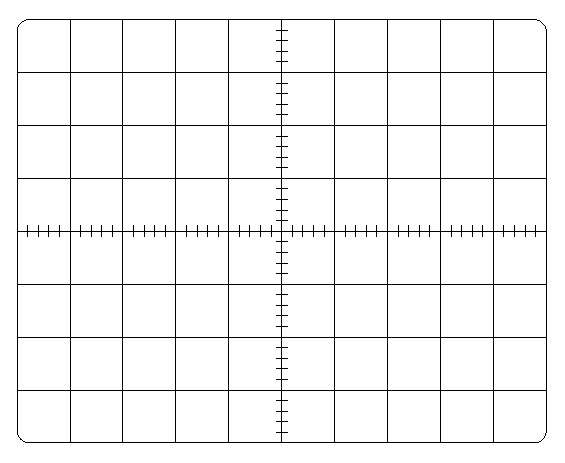
\includegraphics[scale=0.7]{4_oscilloscope/scope.eps} & \hspace{0.5cm} &
\epsfxsize=7cm 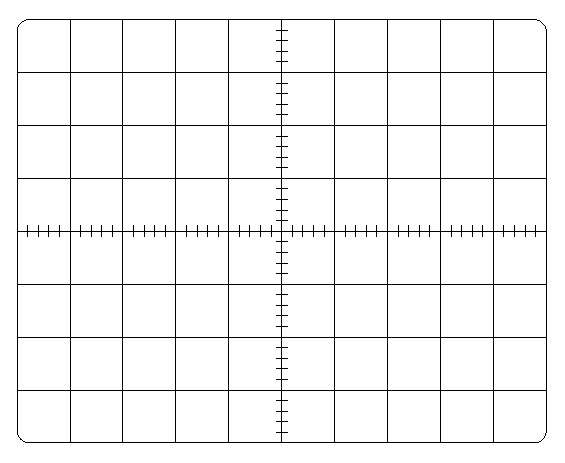
\includegraphics[scale=0.7]{4_oscilloscope/scope.eps}
\end{tabular}\\
\end{center}
\noindent Measure the period $T$ for both waves and the time shift $\Delta t$ between 
them and mark them, in the proper units and with an uncertainty for each, 
below.\\
\ \\
$T$ (ch. 1): \rule{3cm}{.1mm} \hspace*{1cm} $T$ (ch. 2): 
\rule{3cm}{.1mm} \\
\ \\
$\Delta t$: \rule{3cm}{.1mm} \\
\ \\
\ \\
\noindent Now set the phase shifter to its {\bf maximum} value and repeat the above sketch and 
measurements.

\ \\\begin{center}
\begin{tabular}{ccc}
\epsfxsize=7cm 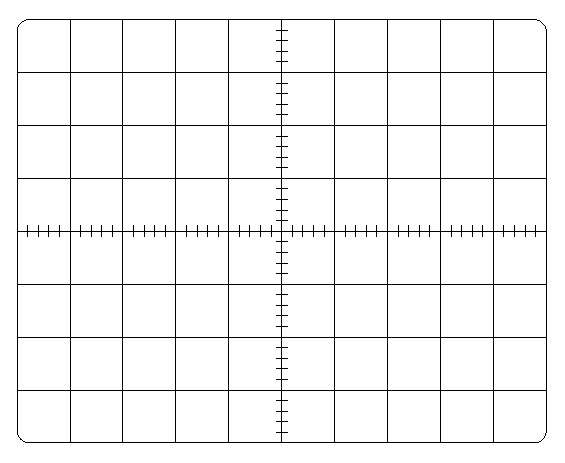
\includegraphics[scale=0.7]{4_oscilloscope/scope.eps} & \hspace{0.5cm} &
\epsfxsize=7cm 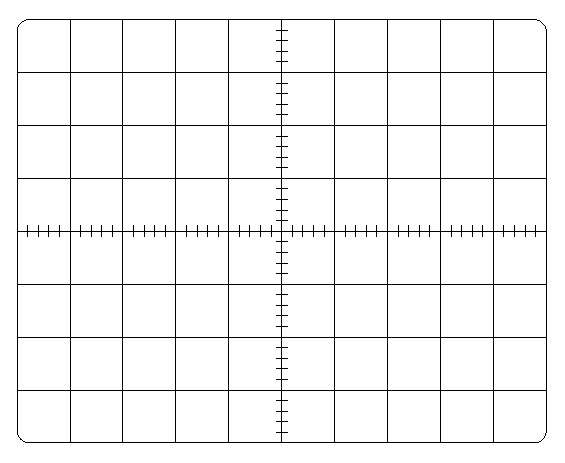
\includegraphics[scale=0.7]{4_oscilloscope/scope.eps}
\end{tabular}\\
\end{center}
$T$ (ch. 1): \rule{3cm}{.1mm} \hspace*{1cm} $T$ (ch. 2): 
\rule{3cm}{.1mm} \\
\ \\  
$\Delta t$: \rule{3cm}{.1mm} \\
\ \\
\ \\


\subsection{Pre-Classroom Check List}
\noindent $\bigcirc$ \hspace*{1cm} Answered questions $\#1-3$. \\
$\bigcirc$ \hspace*{1cm} Sketched 2 waveforms and found their respective 
amplitudes and \\ \hspace*{1.5cm} periods with uncertainties. \\
$\bigcirc$ \hspace*{1cm} Sketched a wave and its phase shifted counterpart on 
the same grid \\ \hspace*{1.5cm} for a minimum shift and found their periods and time shift. \\
$\bigcirc$ \hspace*{1cm} Sketched a wave and its phase shifted counterpart on the same grid
\\ \hspace*{1.5cm} for a maximum  shift and found their periods and time shift. \\



\subsection{In-Classroom Calculations $\&$ Analysis}
\subsubsection{Measuring Amplitude and Frequency}
Calculate frequency from the period of the first waveform measured.  Show your
work for this and every calculation. \\
\ \\
\vskip \baselineskip
\noindent Frequency:  \rule{3cm}{.1mm} \\    
\ \\
\noindent Compare the measured frequency value with the nominal value from the function
generator on your discussion sheet.\\
\vspace*{3cm} \\
\noindent Repeat this calculation to determine the frequency of the second 
waveform measured with the contracted oscilloscope setting. \\
\vspace*{2cm} \\
\noindent Frequency:  \rule{3cm}{.1mm} \\    
\ \\
\noindent How do these values compare
to those made with the ``larger'' signal (the first one you sketched)?  
Specifically, how do the 
uncertainties compare; which are the more precise values?  \\
\vspace*{3cm} \\
\noindent If you require the
most precise measurements possible, what should you make sure to do when you
make measurements with the oscilloscope? \\
\vspace*{2cm}

\subsubsection{Measuring Phase Difference}
%From the two periods obtained, using the {\bf min.} phase shift,  determine 
%the change in period. \\
%\ \\
%$\Delta T$: \rule{3cm}{.1mm} \\
\noindent
Answer the following for the {\bf minimum} setting of the phase shifter.
\ \\
\noindent Are the periods
equal, within uncertainty, {\it i.e.}, has the phase shifter changed the
frequency of the input signal? \\
\ \\
\vspace*{1.5cm} \\
\noindent Now calculate the corresponding phase shift $\phi$ (in radians and degrees) 
with 
uncertainty using equation~(\ref{eq:scope:angphase}).  \\
\vspace*{3cm}\\
$\phi$ (min.) \rule{3cm}{.1mm} \\
\ \\
\vfill

\noindent Now repeat the above for the {\bf maximum.} 
\ \\
\ \\
%\ \\
%$\Delta T$: \rule{3cm}{.1mm} \\ 
\ \\
\noindent Are the periods
equal, within uncertainty, {\it i.e.}, has the phase shifter changed the
frequency of the input signal? \\
\vspace*{3cm}
\\
%\pagebreak
\noindent Calculate the phase shift $\phi$ (in radians and degrees) with 
uncertainty.\\
\vspace*{3cm}\\
$\phi$ (max.) \rule{3cm}{.1mm} \\ 
\ \\
\pagebreak\\
\noindent Now calculate the {\bf range} ($\phi=\phi_{max}-\phi_{min}$) of the
phase shifter with an uncertainty in radians and degrees: \\
\vspace*{2cm}\\
Phase Shift Range: \rule{3cm}{.1mm} \\
\ \\
\noindent Make concluding remarks about the quality of your phase shifter. Does
it function as expected? Compare the range which you calculated above to the
range you expect the shifter to have. Cite all relevant data from your
experiment.

\vfill
\noindent {\Large End Worksheet}



% Go back to ordinary section numbering
\renewcommand{\thesection}{\thechapter.\arabic{section}}















